\chapter{はじめに}
\label{chap:introduction}
\pagenumbering{arabic}

\section{研究背景と目的}
スマートデバイスは, 2010年以降から急速な発展と普及を遂げている.
日本国内における, 近年の情報通信機器の世帯保有状況[1]は, 2010年におけるスマートフォンの保有率が9.7\%, タブレット型端末が7.2\%であるのに対し, 2015年ではスマートフォンが62.6\%, タブレット型端末が21.9\%となっており, 過去5年間でスマートフォンでは6.45倍, タブレット型端末では3.04倍の爆発的普及を実現している.(図1.1参照.)
近年は, 一人でスマートデバイスを複数台所有していることも珍しくない.

\begin{figure}
\begin{center}
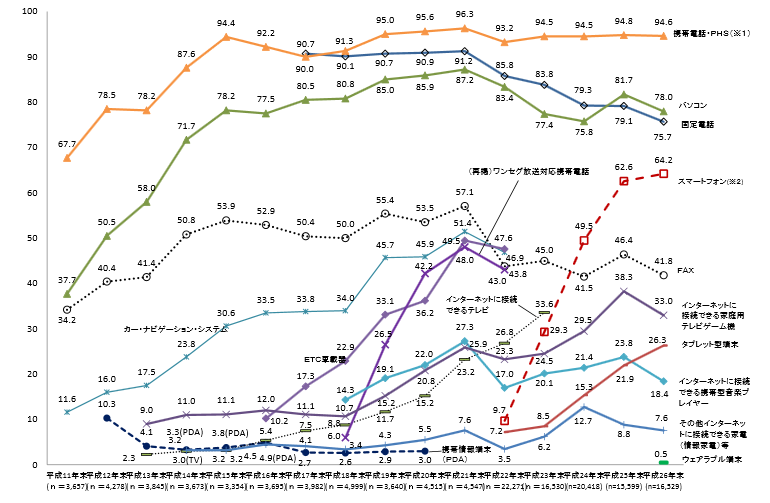
\includegraphics[width=16cm]{fig/n4301010.png}
\end{center}
\caption{情報通信端末の世帯保有数の推移(出典:総務省「平成25年度版 情報通信白書のポイント」)}
\end{figure}

また, スマートフォン, タブレット型端末は, それらが登場する以前に普及していたフィーチャーフォンやPHSとは圧倒的な機能差があり, 非常に多機能なデバイスである.
その多機能性を利用したシステムも数多く開発されており, GPSを利用したナビゲーションシステムや複数端末との通信を利用したソーシャルゲームなど, スマートデバイス普及以前では実現が難しかった様々なシステムが実用化され, 多くのユーザに利用されている.

本研究では, スマートフォン・タブレット型端末のポータビリティの高さとそれらの多機能性に着目し, 「ポータブルデバイスを入力とする情報収集アプリケーションの開発, および収集した情報を解析するWebアプリケーションの開発」を行い, スマートデバイスが収集する情報の正確性, データ解析の速度を調査する.
また, それらを連携させたシステムを試験し, 集積・解析ツールとして利用可能であるかを判定することを目的とする.

ポータビリティに特化しているスマートデバイスが収集し得る情報郡を集積し, それらを解析することによって, 「人々の動きの流れ」や「特定の地域で活動する時間帯」, 「どのような事物に興味を示すのか」など, 多種類の有用な市場情報を獲得することが可能となる.
獲得した情報を適切に利用することで, 市場における現状況の改善や新しい需要の創出等による経済的発展が期待できる.

スマートデバイスで収集可能な多数の情報の中から, 今回は“デバイスで撮影した写真データに記されている文字列”を対象とした情報収集, および収集データの解析を行う.
“画像データ内の文字列”を収集対象としたのは, 「沖縄県が全国有数の観光地である」こと, 「観光客が有名観光地の名称が入った場所で撮影を行う」こと, 「観光客がどの時間帯にどの観光地へ訪れるのかを解析したデータは, 県経済における観光収入の比率が大きい沖縄県において非常に有用な情報となる」ことが主な理由である.

\section{スマートデバイス}
2010年以降から普及しているスマートデバイスであるが, 現在, それらに搭載されている代表的なオペレーティングシステムとして, iOS, Androidが挙げられる.
さらに, タブレット型パーソナルコンピュータの開発, 販売競争も激化しており, 容易に持ち運びが可能なパソコンとしてMicrosoft Windows 10が普及し始めている.

表1.1に, 2013年から2015年にかけての, スマートデバイス用OSの市場占有率[2]のうち, iOS/Android/Windowsの推移を示す.

\begin{table}[htb]
\begin{center}
\begin{tabular}{|l|p{3cm}|p{3cm}|p{3cm}|} \hline
年月 & iOS(\%) & Android(\%) & Windows(\%) \\ \hline \hline
2013年1-3月 & 58.90 & 25.00 & 1.29 \\ \hline
2013年4-6月 & 58.70 & 25.05 & 1.22 \\ \hline
2013年7-9月 & 55.53 & 27.68 & 1.01 \\ \hline
2013年10-12月 & 54.91 & 33.39 & 0.57 \\ \hline
2014年1-3月 & 53.54 & 35.84 & 0.57 \\ \hline
2014年4-6月 & 48.32 & 41.06 & 1.65 \\ \hline
2014年7-9月 & 45.48 & 44.14 & 2.53 \\ \hline
2014年10-12月 & 43.99 & 46.03 & 2.27 \\ \hline
2015年1-3月 & 42.37 & 47.30 & 2.49 \\ \hline
2015年4-6月 & 39.49 & 51.74 & 2.26 \\ \hline
2015年7-9月 & 40.22 & 52.34 & 2.53 \\ \hline
2015年10-12月 & 36.86 & 55.68 & 2.87 \\ \hline
\end{tabular}
\caption{スマートデバイスのオペレーティングシステムの市場占有率の推移}
\end{center}
\end{table}

\subsection{iOS}
iOSとは, Apple Inc.が開発およびリリースしている, iPhone/iPod touch/iPad/iPad mini/Apple TVのオペレーティングシステムである.

2007年6月に発売された初代iPhoneと同時に提供され, 現在でも開発, 提供されている.(表1.2参照.)

\begin{table}[htb]
\begin{center}
\begin{tabular}{|l|l|p{10cm}|} \hline
バージョン & リリース年月 & 対応デバイス \\ \hline \hline
iPhone OS 1.0 & 2007年6月 & iPhone \\ \hline
iPhone OS 1.1 & 2007年9月 & iPhone, iPod touch \\ \hline
iPhone OS 2.0 & 2008年7月 & iPhone/3G, iPod touch \\ \hline
iPhone OS 2.1 & 2008年9月 & iPhone/3G, iPod touch \\ \hline
iPhone OS 2.2 & 2008年11月 & iPhone/3G, iPod touch \\ \hline
iPhone OS 3.0 & 2009年6月 & iPhone/3G/3GS, iPod touch \\ \hline
iPhone OS 3.1 & 2009年9月 & iPhone 3G/3GS, iPod touch \\ \hline
iPhone OS 3.2 & 2010年4月 & iPad \\ \hline
iOS 4.0 & 2010年6月 & iPhone 3GS/4, iPod touch, Apple TV \\ \hline
iOS 4.1 & 2010年9月 & iPhone 3GS/4, iPod touch, Apple TV \\ \hline
iOS 4.2.1 & 2010年11月 & iPhone 3GS/4, iPod touch, iPad/iPad 2, Apple TV \\ \hline
iOS 4.3 & 2011年3月 & iPhone 3GS/4, iPod touch, iPad/iPad 2, Apple TV \\ \hline
iOS 5.0 & 2011年10月 & iPhone 3GS/4/4S, iPod touch, iPad 2, Apple TV \\ \hline
iOS 5.1 & 2012年3月 & iPhone 3GS/4/4S, iPod touch, iPad/iPad 2, Apple TV \\ \hline
iOS 6.0 & 2012年9月 & iPhone 4/4S/5, iPod touch, iPad/Mini, Apple TV \\ \hline
iOS 6.1 & 2013年1月 & iPhone 4/4S/5, iPod touch, iPad/Mini, Apple TV \\ \hline
iOS 7.0 & 2013年9月 & iPhone 4S/5/5C/5S, iPod touch, iPad/Air/Mini/Mini 2, Apple TV \\ \hline
iOS 7.1 & 2014年3月 & iPhone 4S/5/5C/5S, iPod touch, iPad/Air/Mini/Mini 2, Apple TV \\ \hline
iOS 8.0 & 2014年9月 & iPhone 5/5C/5S/6/6 Plus, iPad/Air/Mini/Mini 2, Apple TV \\ \hline
iOS 8.1 & 2014年10月 & iPhone 5/5C/5S/6/6 Plus, iPad/Air 2/Mini/Mini 2/Mini 3, Apple TV \\ \hline
iOS 8.2 & 2015年3月 & iPhone 5/5C/5S/6/6 Plus, iPad/Air 2/Mini/Mini 2/Mini 3, Apple TV \\ \hline
iOS 8.3 & 2015年4月 & iPhone 5/5C/5S/6/6 Plus, iPad/Air 2/Mini/Mini 2/Mini 3, Apple TV \\ \hline
iOS 8.4 & 2015年6月 & iPhone 5/5C/5S/6/6 Plus, iPod touch, iPad/Air 2/Mini/Mini 2/Mini 3, Apple TV \\ \hline
iOS 9.0 & 2015年9月 & iPhone 5/5C/5S/6/6 Plus/6S/6S Plus, iPod touch, iPad/Air 2/Mini 2/Mini 3/Mini 4, Apple TV \\ \hline
iOS 9.1 & 2015年10月 & iPhone 5/5C/5S/6/6 Plus/6S/6S Plus, iPod touch, iPad/Air 2/Mini 2/Mini 3/Mini 4/Pro, Apple TV \\ \hline
iOS 9.2 & 2015年12月 & iPhone 5/5C/5S/6/6 Plus/6S/6S Plus, iPod touch, iPad/Air 2/Mini 2/Mini 3/Mini 4/Pro, Apple TV \\ \hline
\end{tabular}
\caption{iOSのメジャーバージョンと対応デバイスの変移}
\end{center}
\end{table}

iOSの最大の特徴は, Max OS Xと連携が取れる点である.s
iPhoneで撮影した画像や動画をMacに送信し編集する, iPhoneにかかってきた電話をMacで受ける, HandoffでMacで編集していた書類をiOSデバイスで編集するなど, iOSとMac OS Xの高い連携度によって, デバイスに依らない、柔軟性に富んだ作業を実施することが可能となっている.

\subsection{Android}
Androidは, Googleが開発およびリリースしている, Linuxカーネルをベースとした, スマートデバイス用オペレーティングシステムである.

2007年11月にAndroid 1.0が提供され, 現在でも開発, 提供されている.(表1.3参照.)

\begin{table}[htb]
\begin{center}
\begin{tabular}{|l|l|} \hline
バージョン & リリース年月 \\ \hline \hline
Android 1.0 & 2008年9月 \\ \hline
Android 1.1 & 2009年2月 \\ \hline
Android 1.5 Cupcake & 2009年4月 \\ \hline
Android 1.6 Donut & 2009年9月 \\ \hline
Android 2.0 Eclair & 2009年10月 \\ \hline
Android 2.1 Eclair & 2010年1月 \\ \hline
Android 2.2 Froyo & 2010年5月 \\ \hline
Android 2.3 Gingerbread & 2010年12月 \\ \hline
Android 3.0 Honeycomb & 2011年2月 \\ \hline
Android 3.1 Honeycomb & 2011年5月 \\ \hline
Android 3.2 Honeycomb & 2011年7月 \\ \hline
Android 4.0 Ice Cream Sandwich & 2011年10月 \\ \hline
Android 4.1 Jelly Bean & 2012年7月 \\ \hline
Android 4.2 Jelly Bean & 2012年11月 \\ \hline
Android 4.3 Jelly Bean & 2013年6月 \\ \hline
Android 4.4 KitKat & 2013年10月 \\ \hline
Android 5.0 Lollipop & 2014年11月 \\ \hline
Android 5.1 Lollipop & 2015年3月 \\ \hline
Android 6.0 Marchmallow & 2015年10月 \\ \hline
\end{tabular}
\caption{Androidのメジャーバージョンとリリース年月の一覧}
\end{center}
\end{table}

Androidは, Android SDKに対応しているスマートデバイスならば, どれでもそのOSとして無償で利用することが可能である.
また, 他のスマートデバイス向けオペレーティングシステムよりも, ミドルウェアやアプリケーションを作成する際の環境を構築することが容易である.
その高い自由性と対応性により, 2016年現在で最も利用されているスマートデバイス用オペレーティングシステムである.

\subsection{Microsoft Windows 10}
Microsoft Windows 10とは, Microsoft Corporationが開発およびリリースしている, Windowsシリーズに属するオペレーティングシステムである.

1985年11月にWindows 1.0が発表され, 現在でも開発, 提供されている.(表1.4参照.)

Windowsシリーズは, デスクトップ用オペレーティングシステムとしては, 2015年7月時点で約90\%のシェアを誇り, 現在最も利用されているデスクトップ用オペレーティングシステムである.

Windows 8以降は, タブレット型スマートデバイスでも利用することが可能となっており, 持ち運びの便利なタブレット型デバイスにWindows OSを搭載し利用するパソコンユーザも少なくない.

\begin{table}[htb]
\begin{center}
\begin{tabular}{|l|l|l|p{5.5cm}|} \hline
リリースネーム & バージョン & リリース年月 & 特徴 \\ \hline \hline
Windows 1.0 & 1.0 & 1985年11月 & MS-DOSコマンドを入力するのではなく, 画面上をマウスでクリックして動作させる \\ \hline
Windows 2.0 & 2.0 & 1987年12月 & コントロールパネル, キーボードショートカットの導入 \\ \hline
Windows 3.0 & 3.0 & 1990年5月 & プログラムマネージャ, ファイルマネージャ,の導入 \\ \hline
Windows 95 & 4.00 & 1995年8月 & スタートメニュー, タスクバー, ウィンドウの最小化/最大化/閉じるボタンの導入 \\ \hline
Windows 98 & 4.10 & 1998年6月 & コンシューマ向けに設計された初めてのバージョン \\ \hline
Windows 2000 & NT 5.0 & 2000年2月 & ファイル暗号化システム, Windows File Protectionの導入 \\ \hline
Windows ME & 4.90 & 2000年9月 & システム復元機能の導入 \\ \hline
Windows XP & NT 5.1 & 2001年10月 & 二列で構成されたスタートメニュー, タスクバーのタスク結合機能の導入 \\ \hline
Windows Vista & NT 6.0 & 2007年1月 & 透明なウィンドウなどの視覚効果の導入 \\ \hline
Windows 7 & NT 6.1 & 2009年10月 & サムネイルプレビュー, 最近開いたファイルをリスト表示するジャンプリストの導入 \\ \hline
Windows 8 & NT 6.2 & 2012年10月 & タッチスクリーンデバイスへの対応, スタートボタンを廃止し, スタートスクリーンを導入 \\ \hline
Windows 8.1 & NT 6.3 & 2013年10月 & スタートボタンの復活, 最大4つのアプリケーションを並べて使用できる機能の導入 \\ \hline
Windows 10 & NT 10.0 & 2015年7月 & 生体認証テクノロジーの導入 \\ \hline
\end{tabular}
\caption{Microsoft Windowsのメジャーバージョンとリリース年月の一覧}
\end{center}
\end{table}

\begin{figure}[htb]
\begin{center}
\begin{tabular}{c}

\begin{minipage}{0.5\hsize}
\begin{center}
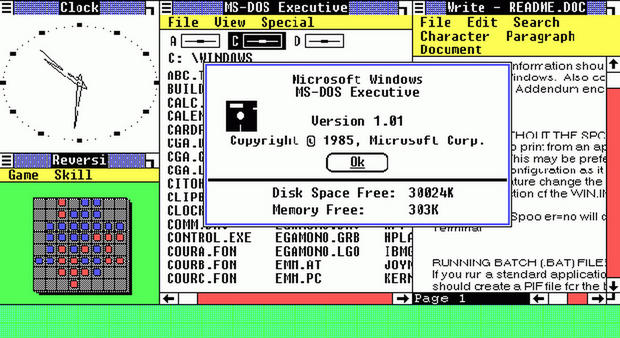
\includegraphics[width=7.5cm]{fig/windows1.jpg}
\caption{Windows 1.0のデスクトップ画面}

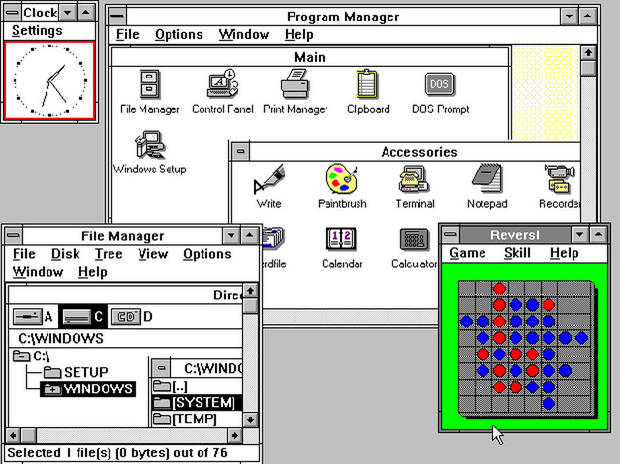
\includegraphics[width=7.5cm]{fig/windows3.jpg}
\caption{Windows 3.0のデスクトップ画面}

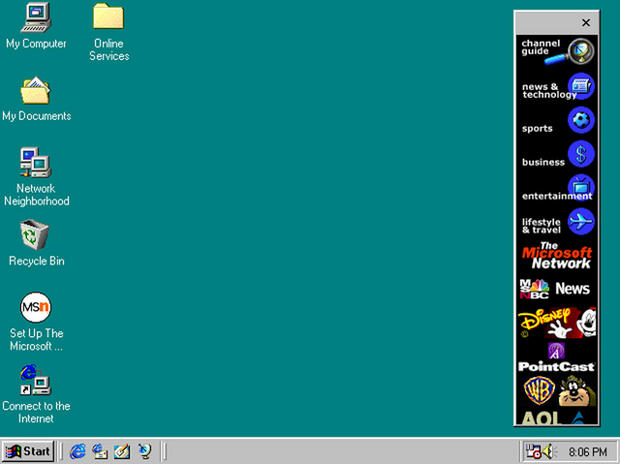
\includegraphics[width=7.5cm]{fig/windows98.jpg}
\caption{Windows 98のデスクトップ画面}
\end{center}
\end{minipage}

\begin{minipage}{0.5\hsize}
\begin{center}
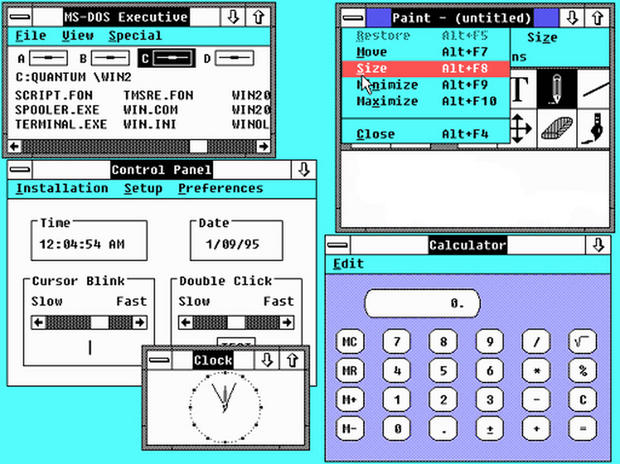
\includegraphics[width=7.5cm]{fig/windows2.jpg}
\caption{Windows 2.0のデスクトップ画面}

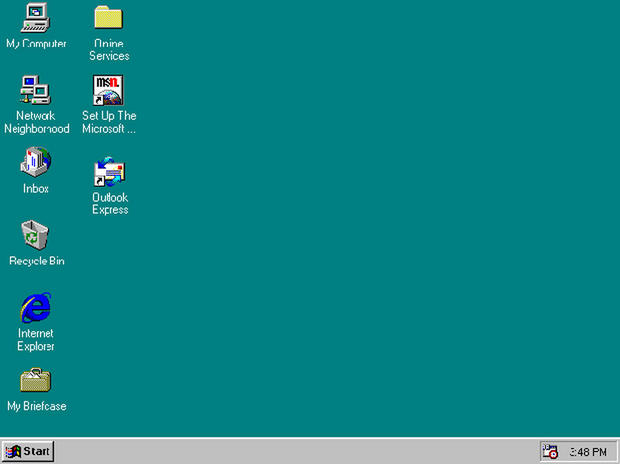
\includegraphics[width=7.5cm]{fig/windows95.jpg}
\caption{Windows 95のデスクトップ画面}

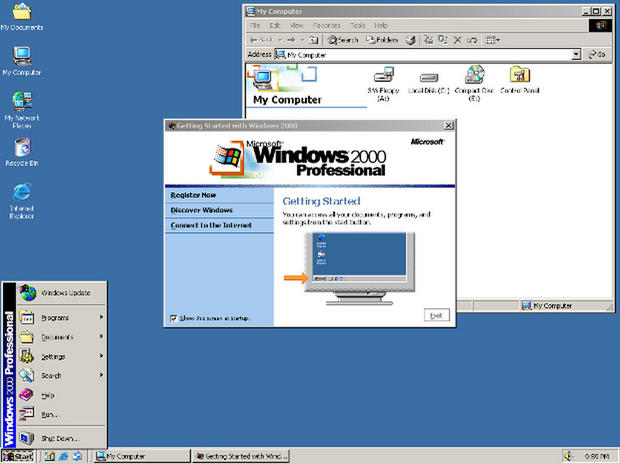
\includegraphics[width=7.5cm]{fig/windows2000.jpg}
\caption{Windows 2000のデスクトップ画面}
\end{center}
\end{minipage}

\end{tabular}
\end{center}
\end{figure}

\begin{figure}[htb]
\begin{center}
\begin{tabular}{c}

\begin{minipage}{0.5\hsize}
\begin{center}
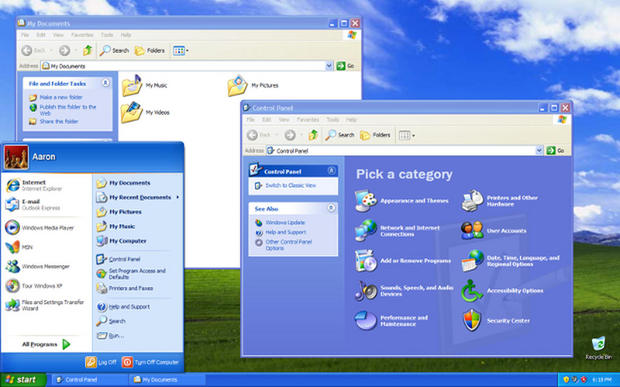
\includegraphics[width=7.5cm]{fig/windowsXP.jpg}
\caption{Windows XPのデスクトップ画面}

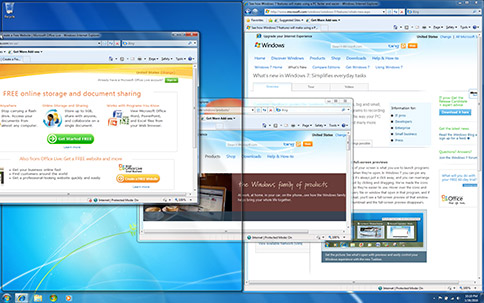
\includegraphics[width=7.5cm]{fig/windows7.jpg}
\caption{Windows 7のデスクトップ画面}

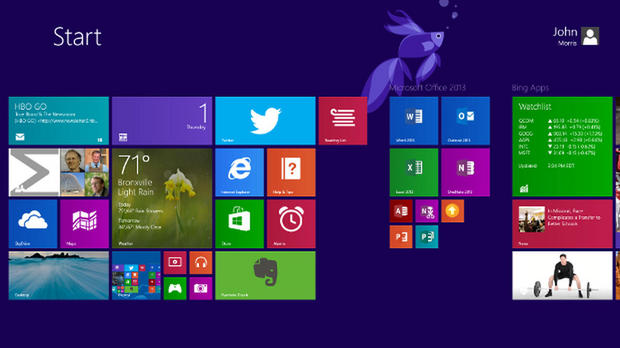
\includegraphics[width=7.5cm]{fig/windows8_1.jpg}
\caption{Windows 8.1のデスクトップ画面}
\end{center}
\end{minipage}

\begin{minipage}{0.5\hsize}
\begin{center}
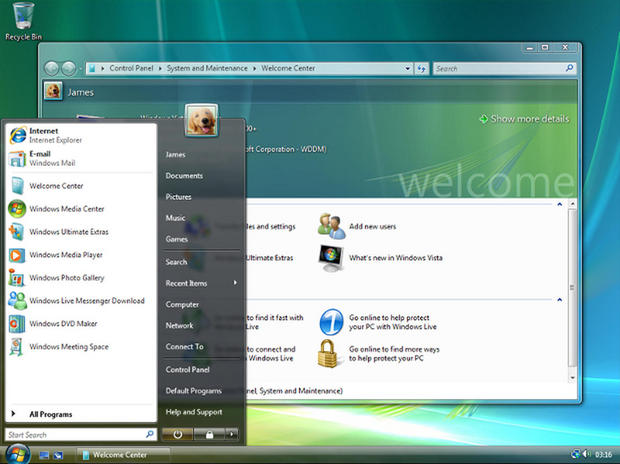
\includegraphics[width=7.5cm]{fig/windowsVista.jpg}
\caption{Windows Vistaのデスクトップ画面}

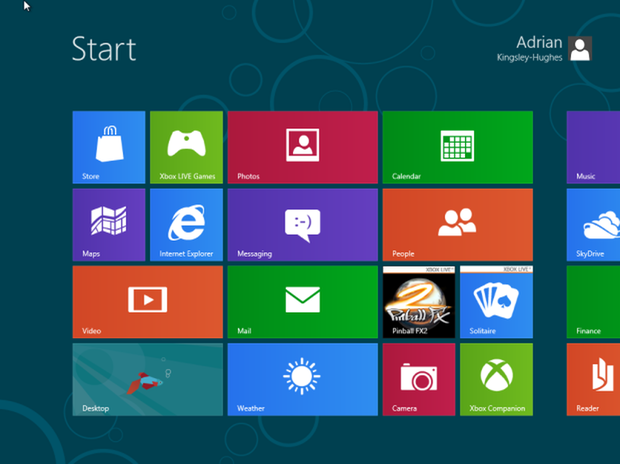
\includegraphics[width=7.5cm]{fig/windows8.png}
\caption{Windows 8のデスクトップ画面}

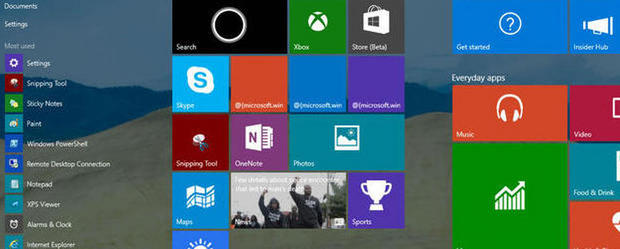
\includegraphics[width=7.5cm]{fig/windows10.jpg}
\caption{Windows 10のデスクトップ画面}
\end{center}
\end{minipage}

\end{tabular}
\end{center}
\end{figure}

\subsection{本研究で使用するスマートデバイス用オペレーティングシステム}
本研究では, 使用するスマートデバイス用オペレーティングシステムをiOSとする.

その理由として, 以下を挙げる.

\begin{itemize}
\item ポータビリティの高さ

iOSデバイスは, スマートデバイスでは現在2位の市場占有率を誇り, そのポータビリティはデータの回収に高い信頼性があると判断した.

\item 開発環境の構築の容易さ

琉球大学工学部情報工学科では, 講義にMacbookを使用しており, iOS/OS X用アプリケーションの開発ツールスイーツであるXcodeとObjective-Cのリファレンスなど, iOSデバイスのアプリケーションを作成するための環境を構築することが容易であるため.

また, 講義でiOSアプリケーションの開発言語であるObjective-Cを学んだことも, iOSデバイスを使用する要因の一つである.
\end{itemize}

\section{論文の構成}
本論文では, 第二章「技術概要」にて本研究にて使用したプログラミング言語やライブラリを解説する.

第三章「実験」では, どのようにしてiOSアプリケーションとWebアプリケーションが連携しているのかを示す.

第四章「本研究の利用例, 利用アイデア」では, 本研究をどのように活かせるのかを考察する.
